\chapter{Electric field}
\section{E and F}
\begin{definition}{E-field, E-field strength}{efield}
	An electric field is a \it{region of space} where a charge experiences an
	electric force.

	Electric field strength \(E\) is the electric force per unit charge
	acting on a \it{positive charge} placed at a point.
	\[\va{E} = \f{\va{F}}{q} = -\odv{V}{r}\]
\end{definition}
\(E\) within a conductor equals \(0\).

\(\va{E}\)-field lines
\begin{itemize}
	\item direct from higher potential (more positive) to lower potential (more negative)
	\item are proportional to the magnitude of the charge
	\item do not intersect
\end{itemize}
\begin{figure}[htpb]
	\centering
	\begin{minipage}{.32\textwidth}
		\centering
		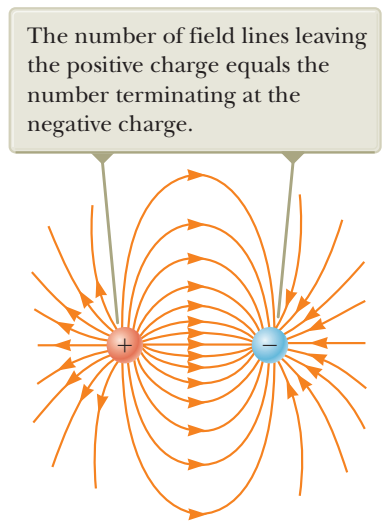
\includegraphics[width=.97\textwidth]{assets/q-minus-q.png}
		\caption{two opposite point charges}
	\end{minipage}
	\begin{minipage}{.32\textwidth}
		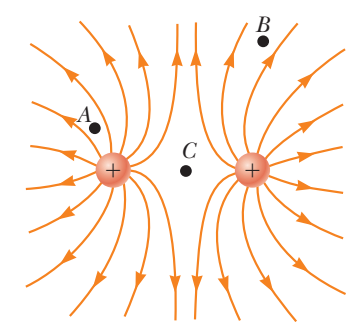
\includegraphics[width=.97\textwidth]{assets/q-q.png}
		\caption{two positive point charges}
	\end{minipage}
	\begin{minipage}{.32\textwidth}
		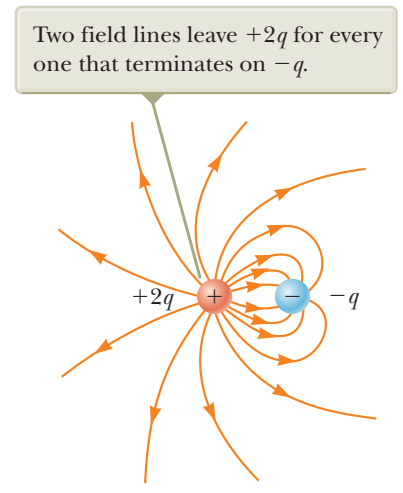
\includegraphics[width=.97\textwidth]{assets/2q-minus-q.png}
		\caption{two opposite point charges \(+2q\) and \(-q\)}
	\end{minipage}
\end{figure}

\begin{definition}{Coulomb's law}{eforce}
	Magnitude of the electric force between two point charges is
	\begin{enumerate}
		\item directly proportional to the product of the magnitude of the charges
		\item inversely proportional to the square of the distance between them
	\end{enumerate}
	\[F = \f{q_1q_2}{4\pi\epsilon_0r^2}=-\odv{U}{r}\]
	\(\epsilon_0 = \) permittivity of free space
\end{definition}

\section{U and V}
\begin{definition}{Electric potential energy}{epe}
	Work done by an external force in assembling a system of charges
	\it{originally at infinity}, with \it{no change in k.e.}
	\begin{align*}
		U                        & = \f{q_1q_2}{4\pi\epsilon_0r}  \\
		U\text{ (by ext. force)} & = U\text{ (by electric force)}
	\end{align*}
	for multiple charges, \(U = \sum_{\forall i,j}U_{ij}\)
\end{definition}
\begin{definition}{Electric potential}{epotential}
	Work done \it{per unit charge} by an ext.~force in bringing a small positive test charge
	from infinity to a point within an electric field, with \it{no change in k.e.}
	\begin{align*}
		V & = \f{U}{q} = \f{q}{4\pi\epsilon_0r}
	\end{align*}
\end{definition}
The change in potential energy\sidenote{work done by \bf{ext.~agent}!} in moving a charge from a
point of potential \(V_i\) to another point of potential \(V_f\) is \(\Delta U = q\ab(V_f - V_i)\).

\(V\) within a conductor is constant.

\bf{Equipotential lines}
\begin{itemize}
	\item distance between lines \(\propto\) \(\va{E}\)-field strength
	\item are perpendicular to \(\va{E}\)-field lines
\end{itemize}
\begin{figure}[htpb]
	\centering
	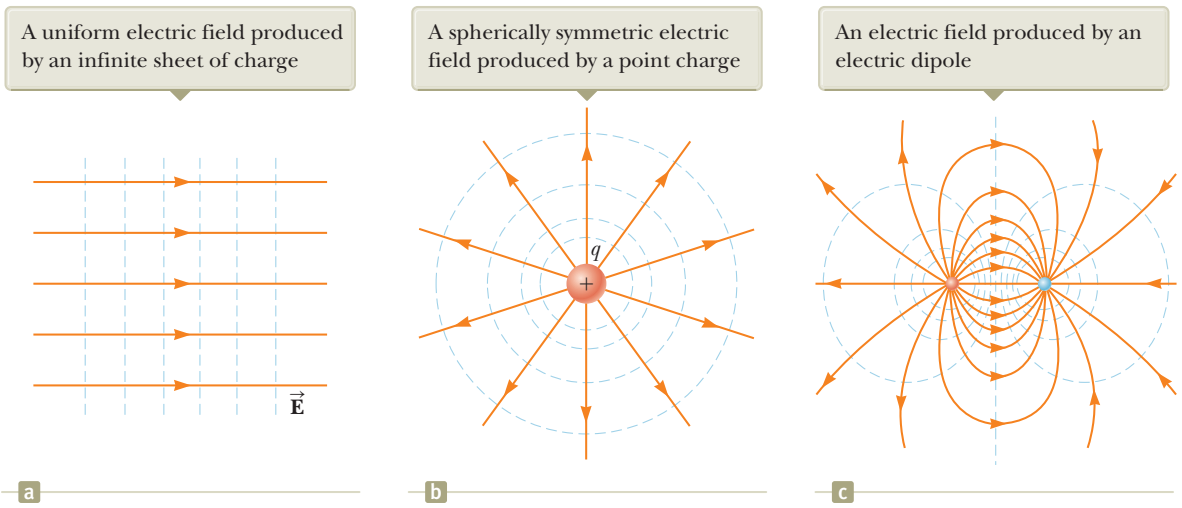
\includegraphics[width=.9\textwidth]{assets/v-lines.png}
	\caption{Equipotential lines and \(\va{E}\)-field lines}
	\label{fig:v-lines}
\end{figure}

A \bf{uniform electric field} is one where the \(\va{E}\)-field strength is the same at all points.
For a potential difference \(V\) applied across a distance \(d\),
\[E = \f{V}{d}\]
\begin{marginfigure}
	\centering
	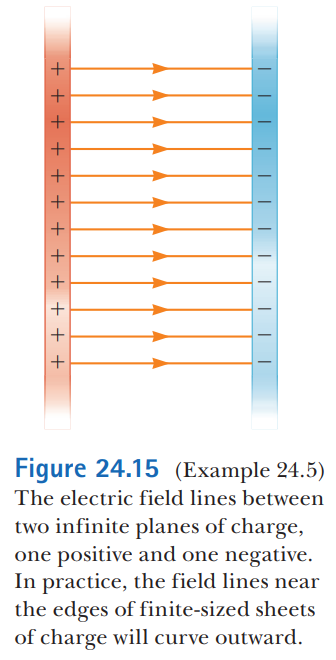
\includegraphics[width=.5\textwidth]{assets/uniform-efield.png}
	\caption{Uniform electric field}
	\label{fig:uniform-efield}
\end{marginfigure}

\begin{marginfigure}
	\centering
	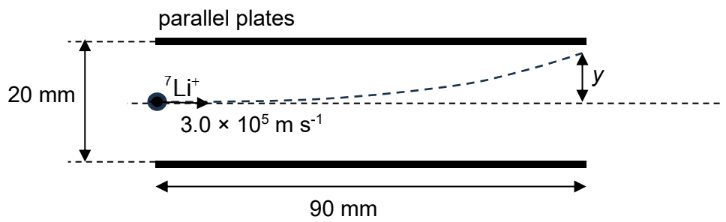
\includegraphics[width=.9\textwidth]{assets/accelerating-li.png}
	\caption{Accelerating \ce{Li+} ion}
	\label{fig:accel-li}
\end{marginfigure}
\begin{example}{}{accelerating-charge}
	\Cref{fig:accel-li} where a \ce{^7Li+} ion (\(m\), \(q\)) is accelerated with a initial
	horizontal velocity \(\va{u}\) through an electric field created by a
	potential difference \(V\) applied over two charged plates of length \(L\),
	separated by distance \(d\). \it{What is the vertical deflection \(y\) of the ion?}

	Since there are no ext.~forces, energy is conserved. We can use the kinematic equations.
	By N2L, \(ma = qE \implies a = \lf{qE}{m} = \lf{qV}{md}\).
	\begin{align*}
		y & = u_yt + \f{1}{2}a_yt^2                 \\
		  & = 0 + \f{1}{2}\f{qV}{md}\ab(\f{L}{u})^2 \\
		  & = \f{qL^2V}{2mdu^2}
	\end{align*}
\end{example}

\section{Summary}
\begin{figure}[htpb]
	\centering
	\input{assets/e-summary.tikz}
	\caption{Summary of electric field}
	\label{fig:e-summary}
\end{figure}
